\section{}
Consider the flow of an incompressible Newtonian fluid between two parallel plates that are 4 mm apart. 
If the upper plate moves to the right with \(u_1 = 5 \, \text{m/s}\) while the bottom one moves to the left with 
\(u_2 = 1.5 \, \text{m/s}\), what would be the net flow rate at a cross-section between the two plates? Take the plate 
width to be 5 cm.

\begin{figure}[h]
    \centering
    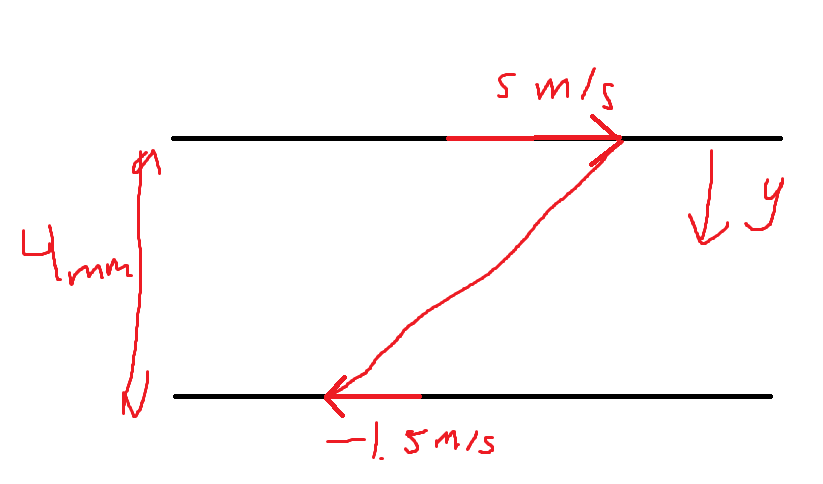
\includegraphics[width=0.5\linewidth]{Questions/Figures/Q3ProblemDiagram.png}
    \caption{Flow between two parallel plates.}
    \label{fig:Q3}
\end{figure}

\subsection{}
Assumptions
\begin{enumerate}
    \item Steady flow
    \item Incompressible flow
    \item No slip at the boundaries
\end{enumerate}

First, denote $y$ as the direction normal to the top plate to the bottom plate. Given the boundary conditions, the velocity
profile is linear, and is given by:

\[
\begin{aligned}
    u(y) &= \frac{u2 - u1}{h}(y) + u_1 \nonumber \\
    &= \frac{-1.5 - 5}{0.004}y + 5 \nonumber \\
    %&= \qty{-1625y + 5}{\meter\per\second} \nonumber
    &= -1625y + 5 \nonumber \;[\unit{\meter\per\second}]
\end{aligned}
\]

The net flow rate of a cross-section between the two plates is given by the integral of the velocity profile times width at 
the cross-section:
\[
    \begin{aligned}
        Q &= \int_{0}^{0.04} u(y)w \, dy \nonumber \\
        &= \int_{0}^{0.04} (-1625y + 5)(0.05) \, dy \nonumber \\
        &= 0.00035 \\
        &= \boxed{\qty{3.50e-4}{\meter\cubed\per\second}}
    \end{aligned}                       
\]


